\section{Orilla}

The planet the campaign takes place on is known as Orilla. Orilla is vastly larger than Earth. It is made of large continents that span a huge ocean. The area of land mass is about six times that of Earth. For this reason, there is a large separation between different regions. Orilla is rich in neutronium which plays a pivotal role in the technological advancements of the time of the Celestials. The climate of Orilla varies based on location. The southern regions are colder but most area's are tropical and mountainous. There are some desert regions in the north east.

The majority of the planet is water. There are many volcanic fault lines all throughout the ocean which form a tunnel system under the mantel. There are volcanoes all around the planet as the size and make-up of the planet causes the inside to be greatly unstable. Storms on the planet can be much more significant and intense than those that would be found on Earth due to its size. The wind is generally calm but storms can last significantly longer and sometimes months. Due to the large variety and length storms can have, this makes travel between islands and larger regions difficult.

Orilla is largely composed of large islands (roughly the scale of Alaska). There is a southern ice region but a warm northern region. There is one large continent with a huge sea in the middle of it.

\begin{center}
	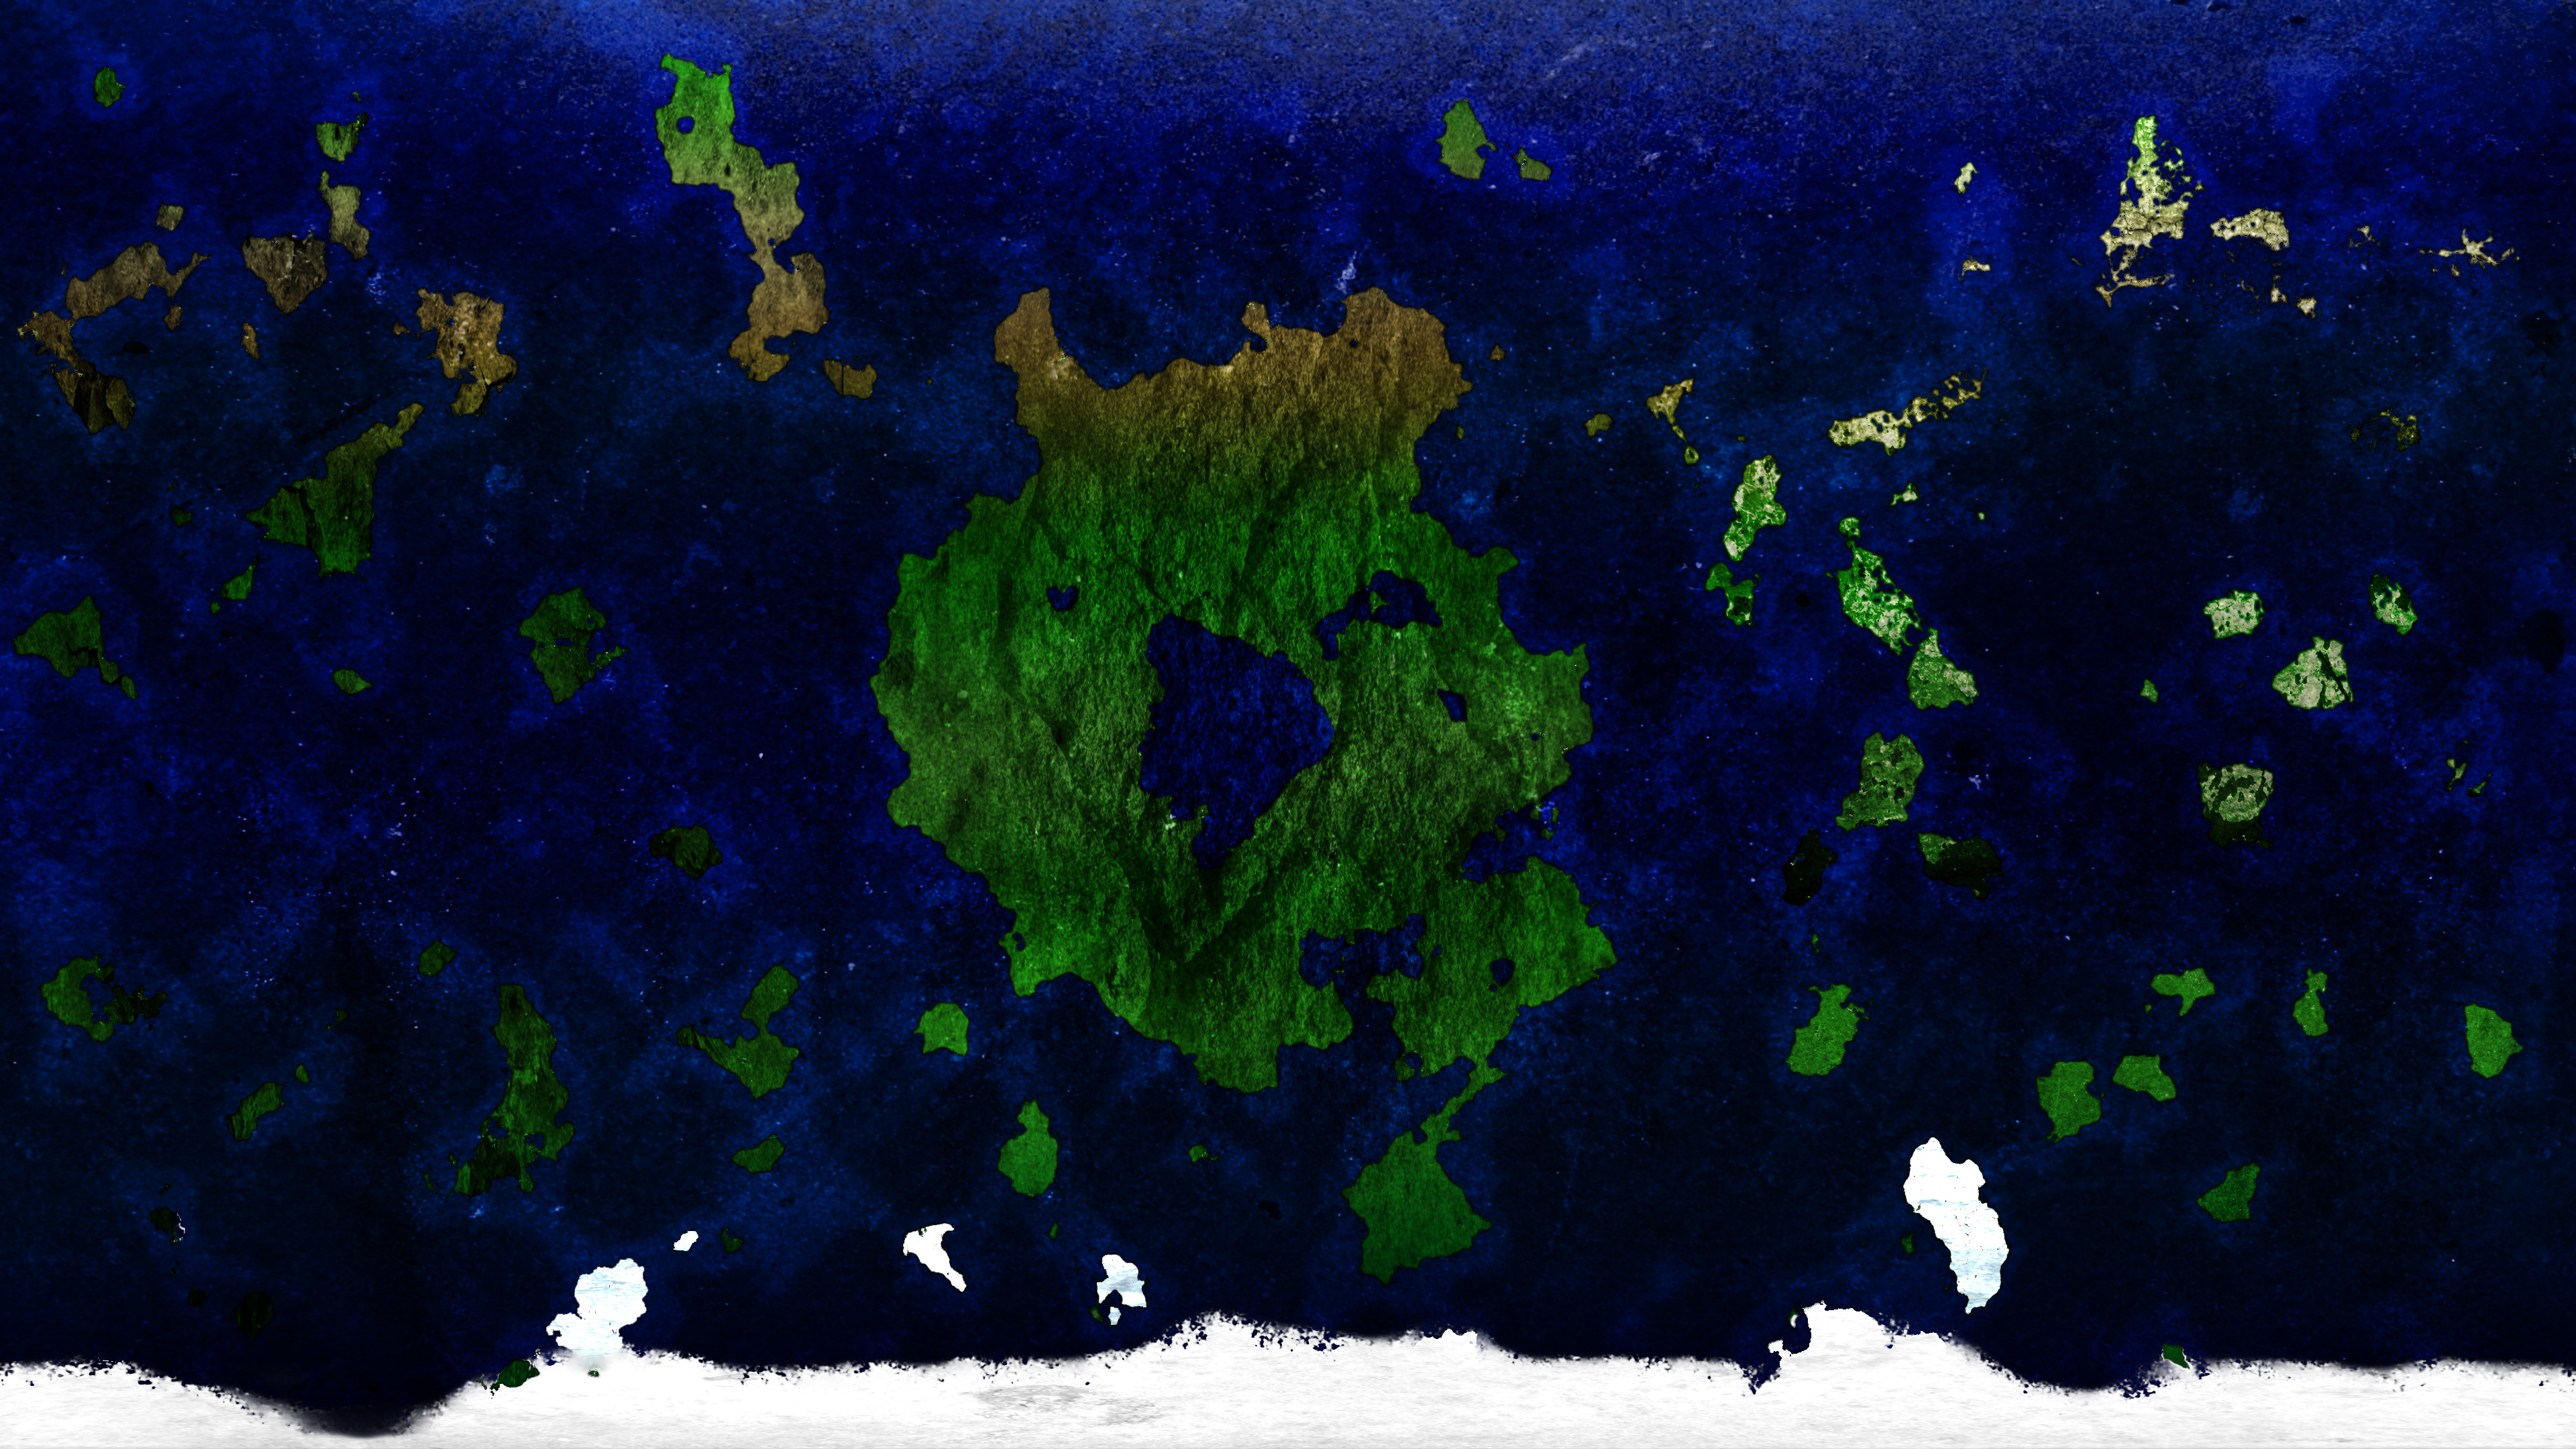
\includegraphics[width=\linewidth]{img/maps/Orilla.jpg}
	
	{\textbf{Orilla:} The massive planet of Orilla}
\end{center}

\begin{center}
	\includegraphics[width=0.7\linewidth]{img/maps/Orilla_SE.jpg}
	
	{The south eastern region of Orilla.}
\end{center}

\subsection{Regions}

The various regions of Orilla are all surrounded by water which gives them (in most cases) fertile land that is good for development of civilization. The regions are generally very large and each unique in many ways.

\subsubsection{Azeroth}

Azeroth is the home of the humans. It appears over time, the humans mainly settled in this region though they can be found in other areas. The most well known cities of this region are Tempestas which is a vast trading city that has sea ports leading to many other regions. 

\subsubsection{Degobah}

This region is similar to the Degobah planet found in Star Wars. It is largely swamp, marsh, and forest with few large mountains. The terrain is relatively smooth as far as elevation but with small hills throughout the entire region. There are many creatures here that cannot be found anywhere else on Orilla. Most of the creatures here are use to warm humid places. 

\subsubsection{Kalimdor}

Kalimdor is a largly forested and mountainous region with many different species and cultures throughout. The region is known for it's large forests and a few vast plains. It also contains some swamps, marshes, and many large cities.

\subsubsection{Tel'Drassil}

Tel'Drassil is the home of the night elves. The island is extremely dense with forest and nature and contains a unique lush type of Asheville trees that do not grown in any other region on Orilla. Tel'drassil contains a world tree which encompasses the majority of its land mass. The tree is home to the elves.

\subsubsection{Abydos}

Abydos is a largely desert region with many ancient pyramids, temples and other ancient structures. The region has farmland to the north and in small areas throughout.

\subsubsection{Vulcan}

Vulcan consists of deserts and mountainous regions. There are many areas of wilderness and some extremely rocky terrain areas.

\subsubsection{Tatooine}

This region is largely desert. This is one of the driest regions in Orilla with almost zero humidity in some areas.

\subsubsection{Korriban}

Korriban is mostly dessert and buried history. The region is extremely windy and mountainous. There is little vegetation due to the regions past. The region contains many old temples and ruins from ancient times. There are also pyramids and large skeletal corpses scattered throughout the land. 

%\subsubsection{Krypton}

%\subsubsection{Sahal}

%\subsubsection{Tuchanka}

\subsubsection{Pandora}

This is the largest land mass on Orilla.

%\subsubsection{Babylonia}

\subsubsection{Vagonbrei}

Vagonbrei is a largely iced over region that is home to many large winter beasts and creatures not found in other regions.

\subsubsection{Statu}

Statu is one of the most underpopulated lush region on all of Orilla. The entire island is largely surrounded by sheer mountainous cliffs which make it difficult to travel deep into. 

%\subsubsection{Telos}

%\subsubsection{Nibiru}

\subsubsection{Kashyyyk}

This area is a mix of mountainous region, beaches and mountains. The jungle regions of Kashyyyk are some of the densest in all of Orilla.

%\subsubsection{Castiana}

%\subsubsection{Zebes}

